%-----------------------------------
%-----------------------------------
% Beamer template made by 月栖竹坞
% 2025.10.08
% xelatex
%-----------------------------------
%-----------------------------------

\documentclass{beamer}

\mode<presentation> {
	\usetheme{Madrid}
	\usecolortheme{rose}
}

\usepackage{graphicx}
\usepackage{booktabs}
\usepackage[UTF8,noindent]{ctexcap}
\usepackage[bookmarks=true]{hyperref}
\usepackage{tabularx}
\usepackage{tikz}
\usetikzlibrary{arrows.meta,positioning,shapes.geometric}

\graphicspath{{nku-thesis-template-2020/figures/}}

\definecolor{accentLine}{HTML}{9A3F78}
\definecolor{muted}{HTML}{666666}
\definecolor{softBlue}{HTML}{F6F0FA}
\definecolor{softGreen}{HTML}{F0F7F3}
\definecolor{softAmber}{HTML}{FFF5E6}
\definecolor{softRed}{HTML}{FCEEEF}
\definecolor{softGray}{HTML}{F8FAFC}
\definecolor{lineGray}{HTML}{DDDDDD}

\setbeamertemplate{caption}[numbered]

\newcommand{\code}[1]{\texttt{\footnotesize #1}}
\newcommand{\tagbox}[2]{%
  \tikz[baseline=(x.base)] \node[rounded corners=2pt, fill=#1, inner xsep=5pt, inner ysep=2.5pt] (x) {\scriptsize\bfseries #2};%
}
\newcommand{\metric}[3]{%
  \begin{beamercolorbox}[wd=\linewidth,sep=0.7em,rounded=true,center]{block body}
    {\Large\bfseries\color{accentLine}#1}\\[-0.2em]
    {\small\color{muted}#2}\\[-0.1em]
    {\scriptsize #3}
  \end{beamercolorbox}
}
\newcommand{\phonepic}[2]{%
  \begin{minipage}{0.31\linewidth}
    \centering
    \includegraphics[height=3.55cm]{#1}\\[-0.2em]
    {\scriptsize\color{muted}#2}
  \end{minipage}
}
\newcommand{\smallcard}[3]{%
  \begin{beamercolorbox}[wd=\linewidth,sep=0.75em,rounded=true]{block body}
    \tagbox{#1}{#2}\par\vspace{0.35em}
    #3
  \end{beamercolorbox}
}

\title[知序答辩]{知序：基于 HarmonyOS 的本地优先学习管理应用}
\author[2413575 柯云超]{2413575\quad 柯云超}
\institute[南开大学]{南开大学计算机学院\\移动应用开发课程设计答辩}
\date{2026 年 6 月}

\begin{document}

%------------------------------------------------
\begin{frame}
  \titlepage
\end{frame}

\begin{frame}
  \frametitle{Overview}
  \tableofcontents
\end{frame}

%------------------------------------------------
\section{项目目标}
\begin{frame}{选题目标：把学习行为串成闭环}
  \begin{columns}[T,onlytextwidth]
    \column{0.54\textwidth}
      \textbf{痛点：}课程资料、任务清单、番茄钟和复盘统计常分散在多个工具里。
      \vspace{0.8em}
      \begin{itemize}
        \item 资料沉淀后不一定能转成行动。
        \item 番茄记录难以回到具体任务和课程项目。
        \item 远程服务不可用时，核心学习流程容易中断。
      \end{itemize}
      \vspace{0.6em}
      \textbf{目标：}用 HarmonyOS 端侧能力实现一个本地优先的学习管理应用。
    \column{0.40\textwidth}
      \metric{5+}{核心页面}{今日、任务、资料、专注、复盘、我的}
      \vspace{0.5em}
      \metric{4 张}{本地 RDB 表}{projects / tasks / pomodoros / study\_resources}
      \vspace{0.5em}
      \metric{2 种}{后端数据库}{MySQL 正式演示，H2 快速测试}
  \end{columns}
\end{frame}

%------------------------------------------------
\begin{frame}{功能闭环：从资料到复盘}
  \begin{center}
    \begin{tikzpicture}[
      node distance=0.16cm,
      flowstep/.style={rectangle, rounded corners=4pt, draw=lineGray, fill=softBlue, minimum width=1.70cm, minimum height=0.85cm, align=center, font=\scriptsize\bfseries},
      arrow/.style={-{Latex[length=2.2mm]}, thick, draw=accentLine}
    ]
      \node[flowstep, fill=softBlue] (res) {资料\\笔记/链接/文件};
      \node[flowstep, fill=softGreen, right=of res] (ai) {AI 提炼\\摘要/要点};
      \node[flowstep, fill=softAmber, right=of ai] (task) {任务\\优先级/子任务};
      \node[flowstep, fill=softRed, right=of task] (focus) {番茄专注\\完成/中断};
      \node[flowstep, fill=softGray, right=of focus] (review) {复盘\\统计/同步};
      \draw[arrow] (res) -- (ai);
      \draw[arrow] (ai) -- (task);
      \draw[arrow] (task) -- (focus);
      \draw[arrow] (focus) -- (review);
      \draw[arrow] (review.south) .. controls +(0,-1.0) and +(0,-1.0) .. node[below, font=\scriptsize, color=muted]{反馈下一轮学习计划} (res.south);
    \end{tikzpicture}
  \end{center}

  \vspace{0.25em}
  \centering
  \phonepic{app-today.jpeg}{今日工作台}
  \hfill
  \phonepic{app-tasks.jpeg}{任务管理}
  \hfill
  \phonepic{app-review.jpeg}{复盘统计}
\end{frame}

%------------------------------------------------
\section{系统设计}
\begin{frame}{技术架构：本地优先 + 后端同步}
  \begin{center}
    \resizebox{0.96\linewidth}{!}{%
      \begin{tikzpicture}[
        node distance=0.55cm and 0.65cm,
        box/.style={rectangle, rounded corners=3pt, draw=lineGray, fill=white, minimum width=3.1cm, minimum height=0.78cm, align=center, font=\scriptsize},
        view/.style={box, fill=softBlue},
        store/.style={box, fill=softGreen},
        data/.style={box, fill=softAmber},
        remote/.style={box, fill=softRed},
        arrow/.style={-{Latex[length=2mm]}, thick, draw=accentLine}
      ]
        \node[view] (ui) {ArkUI 页面\\今日/任务/资料/专注/复盘};
        \node[store, below=of ui] (store) {FocusStore\\状态门面与业务动作};
        \node[data, below left=of store] (rdb) {HarmonyOS RDB\\核心业务数据};
        \node[data, below right=of store] (pref) {Preferences\\登录态/设置/AI 配置};
        \node[store, right=1.35cm of store] (sync) {FocusSyncService\\HTTP 双向同步};
        \node[remote, right=of sync] (server) {Spring Boot\\REST API};
        \node[remote, below=of server] (db) {MySQL / H2\\后端数据库};
        \draw[arrow] (ui) -- (store);
        \draw[arrow] (store) -- (rdb);
        \draw[arrow] (store) -- (pref);
        \draw[arrow] (store) -- (sync);
        \draw[arrow] (sync) -- (server);
        \draw[arrow] (server) -- (db);
      \end{tikzpicture}
    }
  \end{center}
  \vspace{0.3em}
  \begin{block}{分层原则}
    \small
    \begin{itemize}
      \item 视图组件负责展示和交互；\code{FocusStore} 汇聚本地数据并刷新状态。
      \item \code{FocusDatabase} 负责 RDB 建表和 CRUD；后端作为同步与备份增强。
    \end{itemize}
  \end{block}
\end{frame}

%------------------------------------------------
\begin{frame}{端侧数据：RDB 保存学习闭环}
  \begin{table}
    \small
    \begin{tabularx}{\linewidth}{p{2.5cm}p{4.15cm}X}
      \toprule
      表 & 关键字段 & 作用 \\
      \midrule
      \code{projects} & name、color、updated\_at、dirty & 组织课程或学习项目，参与同步。 \\
      \code{tasks} & title、status、priority、client\_request\_id & 保存任务、完成状态、软删除和幂等标识。 \\
      \code{pomodoros} & task\_id、duration、completed、interrupt\_reason & 记录每一次专注结果，支撑复盘统计。 \\
      \code{study\_resources} & title、content、summary、key\_points\_json & 保存资料、AI 摘要和关联任务线索。 \\
      \bottomrule
    \end{tabularx}
  \end{table}

  \vspace{0.2em}
  \begin{block}{设计取舍}
    核心数据优先写入本地 RDB；标签、子任务、资料要点用 JSON 字符串保存，减少课程项目范围内的表结构复杂度。
  \end{block}
\end{frame}

%------------------------------------------------
\section{核心实现}
\begin{frame}{关键流程一：添加任务如何落库并刷新}
  \begin{columns}[T,onlytextwidth]
    \column{0.55\textwidth}
      \begin{tikzpicture}[
        node distance=0.38cm,
        box/.style={rectangle, rounded corners=3pt, draw=lineGray, fill=softGray, minimum width=6.0cm, minimum height=0.58cm, align=center, font=\small},
        arrow/.style={-{Latex[length=2mm]}, thick, draw=accentLine}
      ]
        \node[box, fill=softBlue] (a) {任务页 QuickAddTaskCard 输入};
        \node[box, below=of a] (b) {Index.ets 接收文本或图片草稿};
        \node[box, below=of b] (c) {FocusStore.addTaskFromDraft 构造任务对象};
        \node[box, below=of c] (d) {FocusDatabase.addTask 写入 tasks 表};
        \node[box, below=of d] (e) {FocusStore.refresh 读取最新快照};
        \node[box, fill=softGreen, below=of e] (f) {Index 更新 @State，ArkUI 自动刷新};
        \draw[arrow] (a) -- (b);
        \draw[arrow] (b) -- (c);
        \draw[arrow] (c) -- (d);
        \draw[arrow] (d) -- (e);
        \draw[arrow] (e) -- (f);
      \end{tikzpicture}
    \column{0.40\textwidth}
      \begin{block}{答辩重点}
        这个入口支持多行、截止时间、拍照和上传图片；图片先尝试端侧 OCR，再由 mimo-v2.5 解析为候选草稿，用户确认后再进入本地任务写入流程。
      \end{block}
      \vspace{0.4em}
      \begin{block}{课程知识点}
        \code{@State}、组件传参、异步数据库访问、结果集释放、MVVM 分层。
      \end{block}
  \end{columns}
\end{frame}

%------------------------------------------------
\begin{frame}{关键流程二：专注计时与独立窗口}
  \begin{columns}[T,onlytextwidth]
    \column{0.33\textwidth}
      \centering
      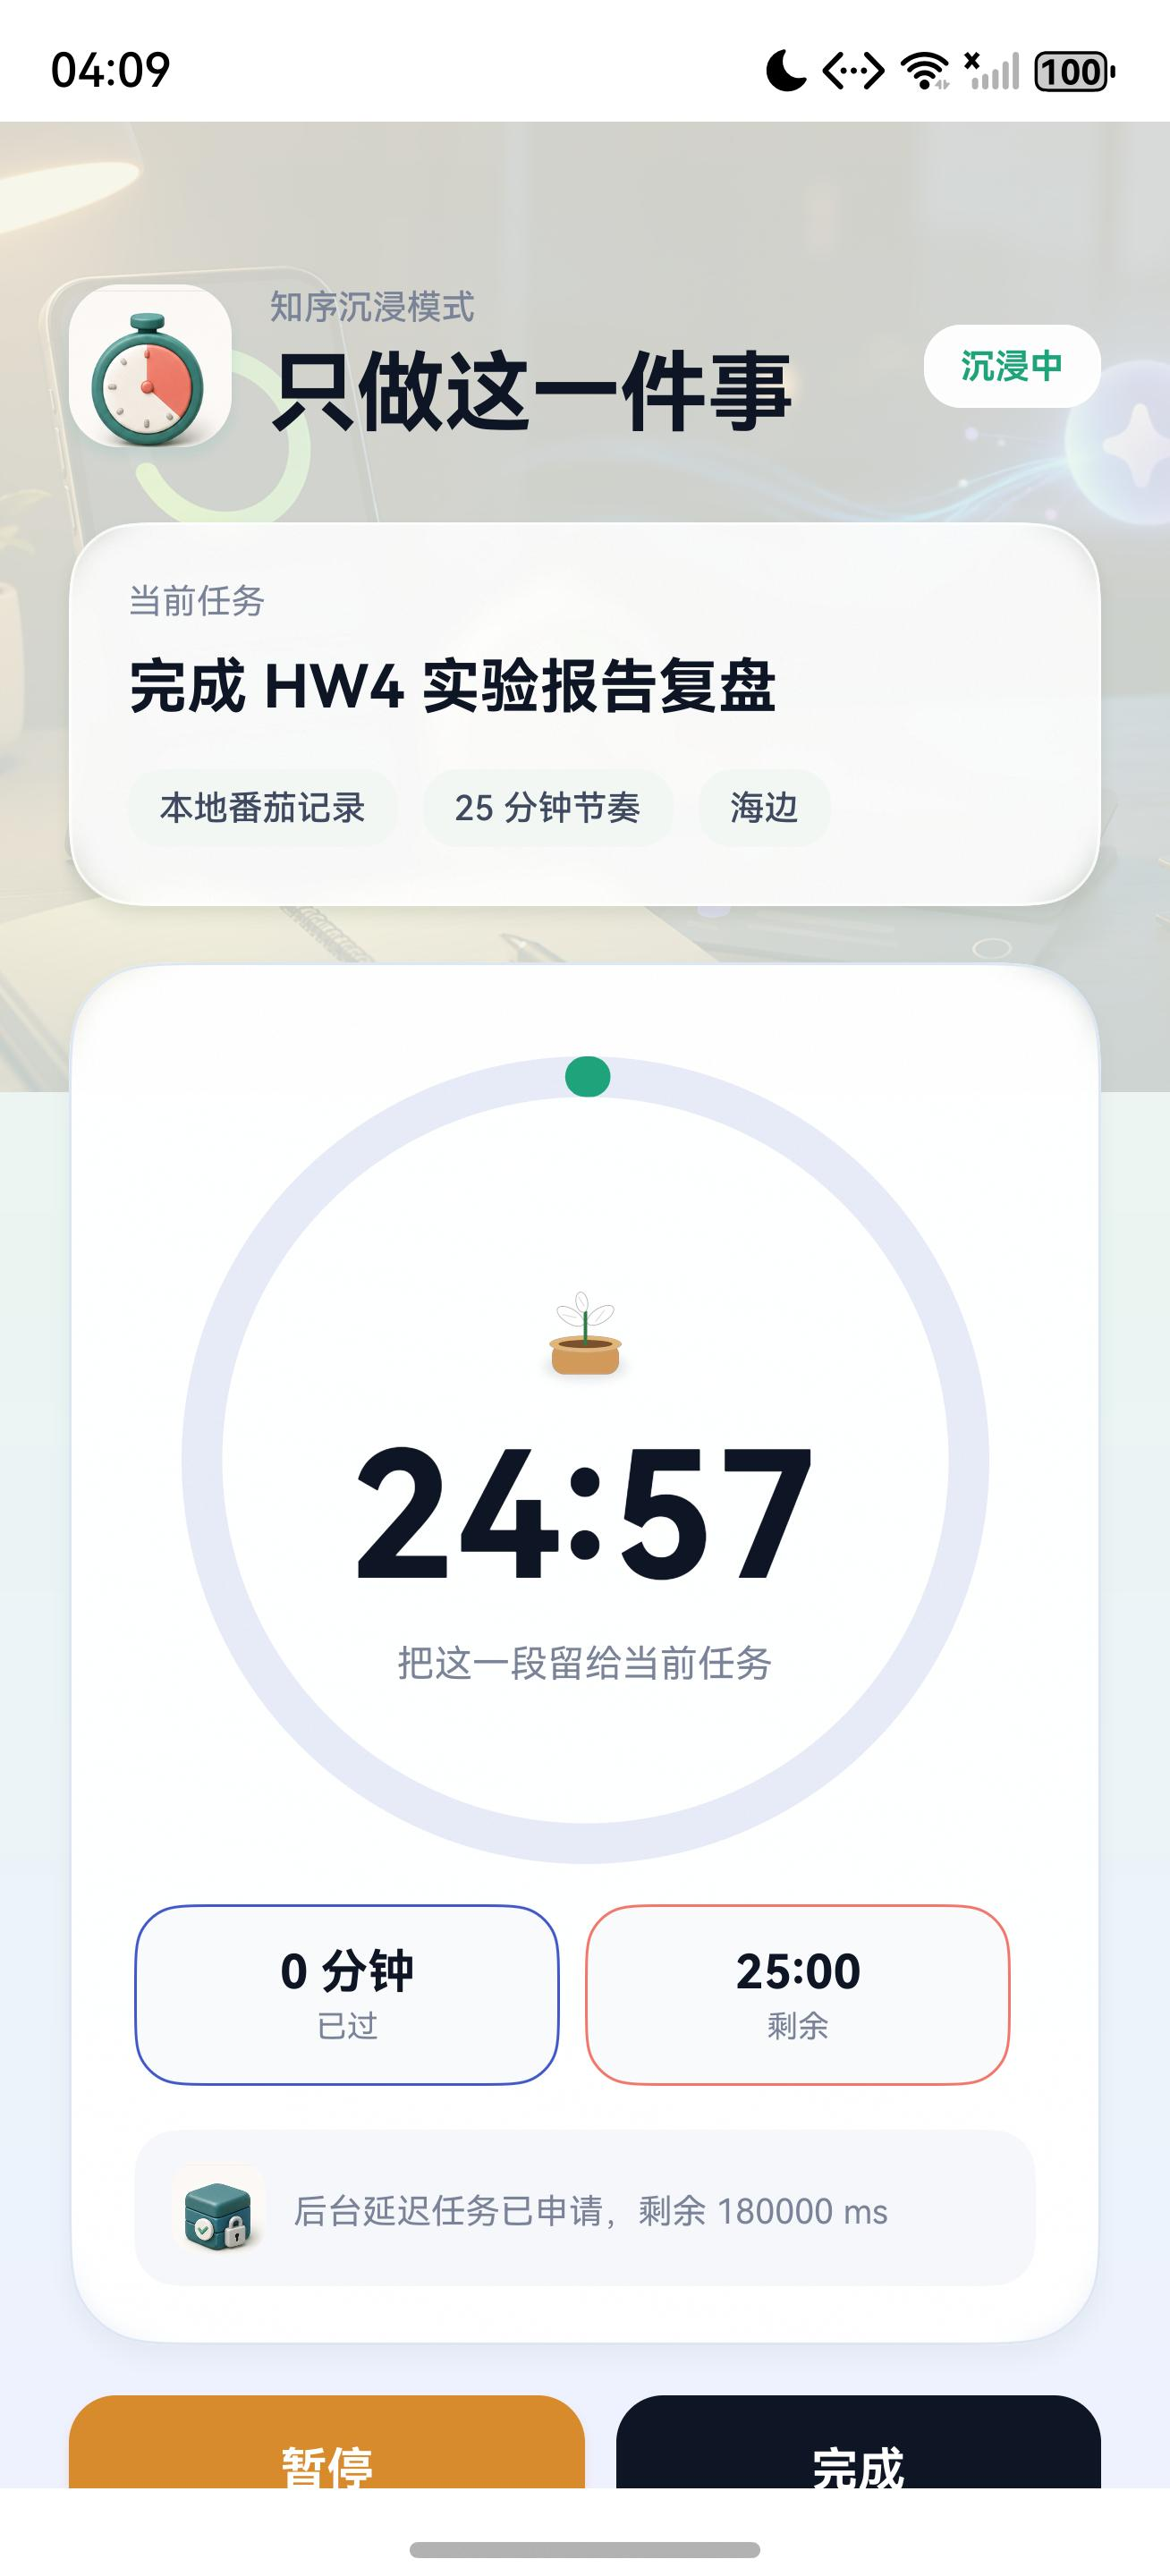
\includegraphics[height=4.25cm]{app-focus.jpeg}\\[-0.2em]
      {\scriptsize\color{muted}专注页运行效果}
    \column{0.62\textwidth}
      \begin{itemize}
        \item 计时器不单纯依赖 \code{setInterval} 每秒减一，而是用 \code{Date.now()} 与开始时间戳计算真实经过时间。
        \item 完成或中断后写入 \code{pomodoros} 表，并更新任务番茄数。
        \item 白噪音通过 \code{AVPlayer} 播放 rawfile 本地音频，停止时释放播放器资源。
        \item \code{FocusAbility} 提供独立沉浸专注窗口，\code{onCreate} 与 \code{onNewWant} 都解析 Want 参数，适配 singleton 热启动。
      \end{itemize}
      \vspace{0.4em}
      \tagbox{softBlue}{UIAbility}
      \tagbox{softGreen}{Want 参数}
      \tagbox{softAmber}{AVPlayer}
      \tagbox{softRed}{RDB 记录}
  \end{columns}
\end{frame}

%------------------------------------------------
\begin{frame}{关键流程三：云同步策略}
  \begin{columns}[T,onlytextwidth]
    \column{0.46\textwidth}
      \centering
      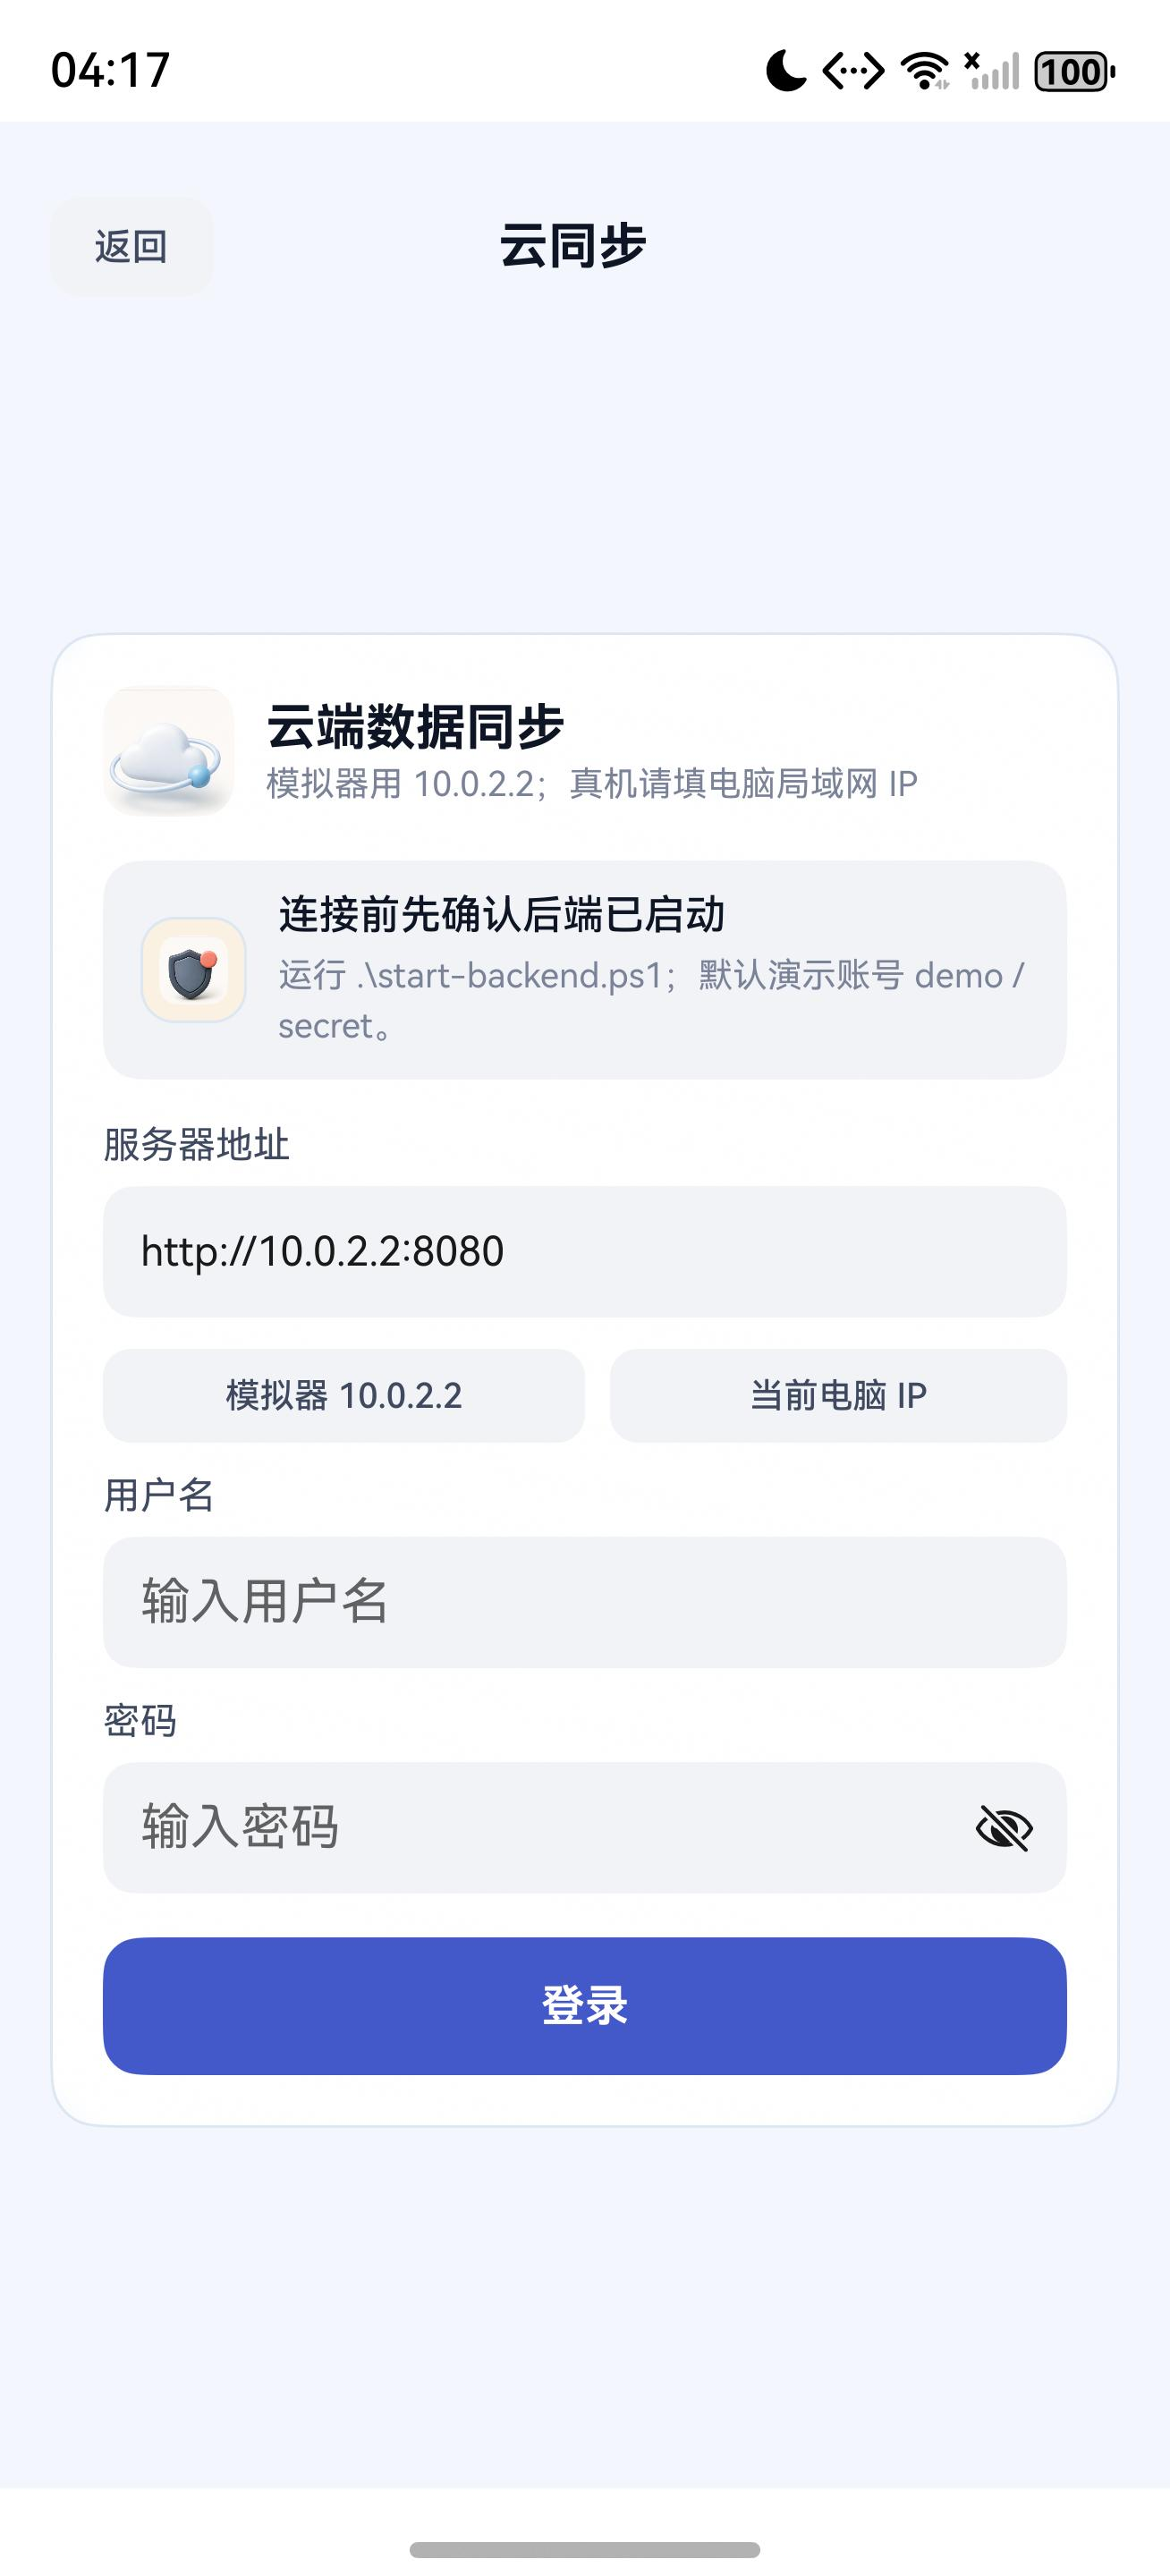
\includegraphics[height=4.15cm]{app-sync.jpeg}\\[-0.2em]
      {\scriptsize\color{muted}云同步页面}
    \column{0.50\textwidth}
      \begin{block}{同步步骤}
        \begin{enumerate}
          \item \textbf{Pull}：按 \code{serverTime} 游标拉取增量数据。
          \item \textbf{Merge}：合并到本地 RDB，按 \code{updatedAt} 判断新旧。
          \item \textbf{Push}：上传本地 \code{dirty = 1} 的项目、任务和番茄记录。
          \item \textbf{Mark}：成功后本地清除 dirty，并保存新的同步游标。
        \end{enumerate}
      \end{block}
      \vspace{0.3em}
      \small
      \tagbox{softBlue}{dirty 增量上推}
      \tagbox{softGreen}{clientRequestId 幂等去重}
      \tagbox{softAmber}{updatedAt 冲突处理}
      \tagbox{softRed}{JWT 鉴权}
  \end{columns}
\end{frame}

%------------------------------------------------
\begin{frame}{课程知识点覆盖}
  \begin{columns}[T,onlytextwidth]
    \column{0.48\textwidth}
      \begin{block}{HarmonyOS 端侧能力}
        \begin{itemize}
          \item \textbf{Navigation}：资料库、复盘、云同步、设置使用真实页面栈。
          \item \textbf{RDB}：\code{FocusDatabase} 建表、CRUD、迁移字段与 ResultSet 释放。
          \item \textbf{Preferences}：保存登录态、AI 配置和专注设置。
        \end{itemize}
      \end{block}
    \column{0.48\textwidth}
      \begin{block}{并发、混合渲染与后端}
        \begin{itemize}
          \item \textbf{TaskPool / ArkWeb}：复盘统计后台快照与 H5 图表。
          \item \textbf{UIAbility}：主入口、独立专注窗口和桌面服务卡片。
          \item \textbf{Spring Boot}：JWT 鉴权、MyBatis 数据访问和同步接口。
        \end{itemize}
      \end{block}
  \end{columns}
\end{frame}

%------------------------------------------------
\section{演示与总结}
\begin{frame}{运行效果与演示路径}
  \centering
  \phonepic{app-resources.jpeg}{资料库}
  \hfill
  \phonepic{app-focus.jpeg}{番茄专注}
  \hfill
  \phonepic{app-profile.jpeg}{我的页面}

  \vspace{0.6em}
  \begin{block}{录屏演示顺序}
    启动 Spring Boot 后端 $\rightarrow$ 打开 HarmonyOS 应用 $\rightarrow$ 登录/本地使用 $\rightarrow$ 添加任务 $\rightarrow$ 开始专注 $\rightarrow$ 查看复盘 $\rightarrow$ 执行云同步。
  \end{block}
\end{frame}

%------------------------------------------------
\begin{frame}{总结与展望}
  \begin{columns}[T,onlytextwidth]
    \column{0.48\textwidth}
      \begin{block}{已完成}
        \begin{itemize}
          \item 原生 HarmonyOS 前端与组件化页面。
          \item 本地 RDB 持久化与学习闭环。
          \item Spring Boot 后端、JWT 鉴权和 MyBatis 数据访问。
          \item 任务、番茄、资料、复盘、云同步等完整演示链路。
        \end{itemize}
      \end{block}
    \column{0.48\textwidth}
      \begin{block}{后续改进}
        \begin{itemize}
          \item 更细粒度的同步冲突合并策略。
          \item AI 资料问答、周报生成和阶段复习计划。
          \item 真机通知、后台计时可靠性与无障碍体验优化。
        \end{itemize}
      \end{block}
      \vspace{0.8em}
      \centering
      {\Huge\bfseries\color{accentLine}谢谢！}\\
      {\large 欢迎老师批评指正}
  \end{columns}
\end{frame}

\end{document}
